%% Use this line for the final version of your report
%\documentclass[final,UKenglish]{include/RaM/RaM-MScReport}

%% Use this line for the draft versions of your report, it enables rro/notes/line numbers/date in footer
\documentclass[lineno,UKenglish]{include/RaM/RaM-MScReport}

\settitle{Development of a myocardial perfusion phantom}
\setauthor{G.J. de Vries, s1854526}
%-------------------------------------------------------------------------------------------------
% This settings.tex contains settings required for *all* documents (reports, presentations, etc)
% Project or Report specific settings should go to their own settings files (eg CE/settings.tex)
% This file is included after the class definition and before project and report specific settings 
%-------------------------------------------------------------------------------------------------

%--------Useful packages (required by the example files, turn off if you do not use them)-------
\usepackage{babel}					% Add language specific support
%\usepackage{makeidx}				% Index support
%\usepackage[totoc,justific=RaggedRight]{idxlayout}	% Make last page of index balanced and add index to toc
\usepackage{caption}				% Provides means to style captions
%\usepackage{subcaption}				% Provides support for (sub)figures and (sub)tables
%\usepackage{float}					% Improved interface for floating objects (eg figures, tables, ...)
\usepackage{enumitem}				% Add styling support to (enumerate) environments
\usepackage{listings}				% Allows (external) source files to be shown in a syntax highlighted way
%\usepackage{amsmath}				% Provides miscellaneous enhancements for documents containing formulas
\usepackage{datetime}				% Provides commands for displaying the current time
%\usepackage{etoolbox}				% Provides \AtBeginEnvironment command
\usepackage{eurosym}				% Defines \euro command to display euro symbols
%\usepackage{appendix}				% Makes it possible to modify appendix numbering
%\usepackage{longtable}				% Allows tables to span multiple pages
%\usepackage{units}					% Shows units (eg m/s) in a nice way
%\usepackage{ctable}				% Provides \ctable command for the typesetting of table and figure floats
%\usepackage{ccaption}				% Support continuation captions (eg multi-page tables)
%\usepackage{verbatim}				% Adds verbatim environment, in which texts are exactly copied to the output
%\usepackage{pdfpages}				% Include PDF pages/documents in the current document
\usepackage{color, colortbl}
\definecolor{Gray}{gray}{0.9}

\usepackage{tabularx}

\usepackage{xfrac}

\usepackage{pdflscape}

\usepackage{multicol}

%%%%%%%%%%%%%%%%%%%%%%%%%%%%%%%%%%%%%%%%%
%%%%%%% Acronyms %%%%%%%%%%%%%%%%%%%%%%%%
\usepackage{acro}

%\DeclareInstance{acro-title}{empty}{sectioning}{name-format =}

\DeclareAcronym{CT}{
	short 	= CT,
	long 	= Computed Tomography,
	class 	= abbrev
}

\DeclareAcronym{MRI}{
	short	= MRI,
	long	= Magnetic Resonance Imaging,
	alt		= MR,
	class 	= abbrev
}

\DeclareAcronym{SPECT}{
	short	= SPECT,
	long	= Single-Photon Emission Computed Tomography,
	class	= abbrev
}

\DeclareAcronym{PET}{
	short 	= PET,
	long	= Positron Emission Tomography,
	class	= abbrev
}

\DeclareAcronym{MPI}{
	short	= MPI,
	long	= Myocardial Perfusion Imaging,
	class	= abbrev
}

\DeclareAcronym{PET-MR}{
	short	= PET-MR,
	long	= PET-Magnetic Resonance,
	class	= abbrev
}

\DeclareAcronym{AIF}{
	short	= AIF,
	long	= Arterial Input Function,
	class	= abbrev
}

\DeclareAcronym{CZT}{
	short	= CZT,
	long	= Cadmium Zinc Telluride,
	class	= abbrev
}

\DeclareAcronym{CAD}{
	short	= CAD,
	long	= Coronary Artery Disease,
	class	= abbrev
}

\DeclareAcronym{VC} {
	short	= VC,
	long	= Vena Cava,
	class	= abbrev
}

\DeclareAcronym{PA}{
	short				= PA,
	long				= Pulmonary Artery,
	long-plural-form 	= Pulmonary Arteries,
	short-plural		= s,
	class	= abbrev
}

\DeclareAcronym{PV}{
	short				= PV,
	long				= Pulmonary Vein,
	long-plural 		= s,
	short-plural		= s,
	class	= abbrev
}

\DeclareAcronym{PMT}{
	short			= PMT,
	short-plural	= s,
	long			= Photomultiplier Tube,
	long-plural		= s,
	class			= abbrev
}
%%%%%%%%%%%%%%%%%%%%%%%%%%%%%%%%%%%%%%%%%%%%%%%%
%%%%%%%%%%%%%%%% END ACRONYM %%%%%%%%%%%%%%%%%%%

\usepackage{include/files/requirements}

\iffinalversion
	\usepackage[final]{include/files/notes}% Add note commands, [final] removes all notes from the document
	\usepackage[final]{include/files/rro}  % Add Rich Report Outline support, [final] removes all RRO output from document
\else
	\usepackage{include/files/notes}       % Add note commands
	\usepackage{include/files/rro}         % Add Rich Report Outline support
\fi

% Add wrongly (or unknown) hyphened words here (space separated and - at possible hyphenation positions):
%\hyphenation{}

%% Spacing possibilities for captions are available as well
% See captions.pdf for all options!
\captionsetup{font=small,labelfont=bf}

%% Center all figures by default
%% http://tex.stackexchange.com/questions/2651/should-i-use-center-or-centering-for-figures-and-tables
\makeatletter
\g@addto@macro\@floatboxreset\centering
\makeatother

%% Make use small font size in verbatim environment
% Note: AtBeginEnvironment is provided by etoolbox package
%\AtBeginEnvironment{verbatim}{\small}

%% Include verbatim in the subfigure env
% From: subfig.pdf, section 4.4
% <Uncomment if verbatim is required in subfloat>:
%\makeatletter
%\newbox\sf@box
%\let\orig@subfloat\subfloat
%\renewenvironment{subfloat}[2][]%
%{ \def\sf@one{#1}%
%  \def\sf@two{#2}%
%  \setbox\sf@box\hbox
%  \bgroup}%
%{ \egroup
%  \ifx\@empty\sf@two\@empty\relax
%    \def\sf@two{\@empty}
%  \fi
%  \ifx\@empty\sf@one\@empty\relax
%    \orig@subfloat[\sf@two]{\box\sf@box}%
%  \else
%    \orig@subfloat[\sf@one][\sf@two]{\box\sf@box}%
%  \fi}
%\makeatother
%% Uncomment till here
  
%% Automatically provide H option for floats
% Requires float package
% \floatplacement{figure}{H} 
% \floatplacement{table}{H} 

%% abbreviation making
\newcommand{\abbr}[1]{(\textit{#1})}

%%lstlisting settings
\lstset{	%aboveskip=20pt,%
		numbers=none, %no line numbers
%		numbers=left, %show line numbers
		numberstyle=\tiny,%
		frame=single,%
		frameround={t}{t}{t}{t},%
		numbersep=5pt,%
%		language=C,% (default) code language in the document
		captionpos=b,%
		xleftmargin=2em,
		framexleftmargin=1.5em,
		xrightmargin=2em,
		framexrightmargin=1.5em,
		morecomment=[s][\itshape]{<}{>}, %also define <> as comment
		morecomment=[s][\itshape]{[}{]} %also define [] as comment
}

%lstinline with empty language definition
\lstdefinelanguage{empty}{}
\newcommand{\mylstinline}[1]{{\lstinline[language=empty]{#1}}}

% Default value of top separator (empty space) of lists
\setlist{topsep=4pt}

%% Don't show warnings like: ``PDF inclusion: found PDF version <1.x>, but at most version <1.4> allowed
% Uncomment if you experience these kind of warnings 
%\ifpdf
%	\pdfminorversion=6 
%\fi

\begin{document}
% Numbered roman style

\makerro				% Build RichReportOutline.rro file

\frontmatter


\includepdf{./frontpage/frontpage_r0d01.pdf}

% Use \maketitle or the available PDF when it is released (for student reports)
\maketitle

% Enter the name of the official RaM title page PDF between the brackets
% ! This method disables the option of using EPS files in your report.
% ! If EPS images are required, use LaTeX source instead of the PDF file
% 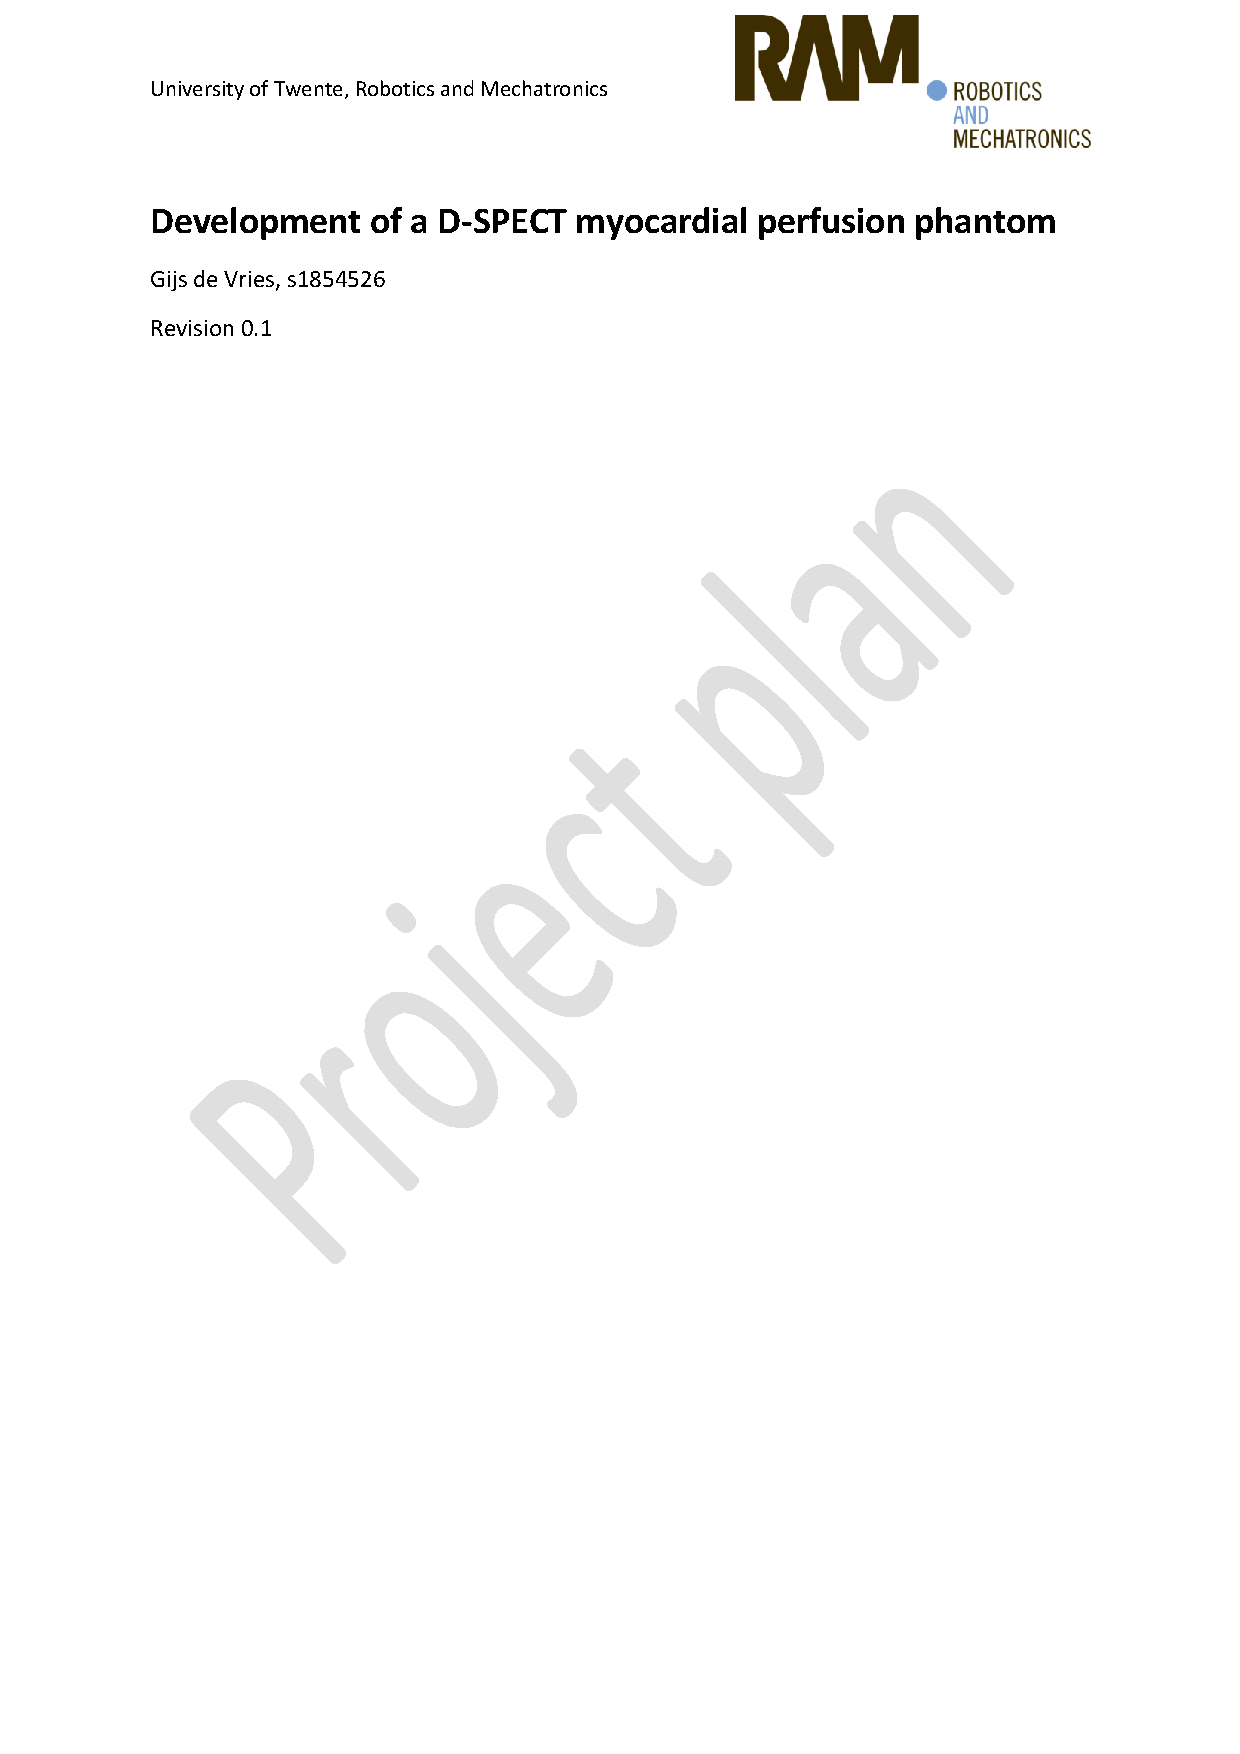
\includepdf{./frontpage/frontpage_r0d1.pdf}
\cleardoublepage

% \include{Summary}
% Dutch summary is not obligatory
%\include{Samenvatting}

\chapter*{Preface}

\vskip-10pt
The system requirements specify all the requirements for the myocardial perfusion phantom. These requirements are based on research and interviews with stakeholders.

\vskip50pt
G.J. (Gijs) de Vries\\
Enschede, 7\textsuperscript{th} of January 2019
%In a two-sided printing style, it makes the next page a right-hand
% (odd-numbered) page, producing a blank page if necessary.
\cleardoublepage

% Add the table of contents pages (TOC)
\tableofcontents

% The report starts here
\mainmatter

% this contains a showcase of LaTeX
\chapter{Introduction}
\label{ch:Intro}

\rrod{Read into background information on D-SPECT}
\rrod{Write global background information}
\rrod{Introduce the rest of the document}
\rrod{Assignment was for dynamic SPECT scanning, but is that the same as using the D-SPECT? The D-SPECT can scan dynamically, and is available in ZGT}
\rrod{Too much SPECT detail in introduction? Moved to literature}
\rrot{Give arguments why to choose SPECT}

\Ac{MPI}, or, simply put, the imaging of the blood flow in the heart muscle, plays an important role in diagnosing heart failure or detecting \ac{CAD}. Imaging systems like \ac{CT}, \ac{MRI}, \ac{SPECT}, or \ac{PET} can visualise a (radioactive) contrast bolus in the supplying arteries and in underlying myocardial tissue, whose flow can give an indication of narrowed or blocked blood vessels.

Many variations in the visualisation process of myocardial perfusion, including variations in hard- and software, can (significantly) influence the outcome and in turn have consequences for patient treatment. These variations need to be validated against a well-known baseline.

The goal of the project is to develop a prototype myocardial perfusion phantom capable of repeated simulations of typical and cardiac defect situations using clinical software commonly used in myocardial perfusion scans. Most software packages require anatomical recognition points which imposes anatomical requirements on the phantom. In addition, the phantom can be used for educational and training purposes to demonstrate the impact of (poorly) chosen variables, e.g. pressure or flow, scanning parameters, cardiac defects, and so forth.

\section*{Document overview}
\label{sec:doc_overview}
\rrod{Update in correspondence with meeting december 10}
The project plan consists of a literature review of existing myocardial perfusion phantoms, their comparison to human physiology, and a discussion between the different types of scanners. The literature is followed by the research methodology containing the research questions and goals of the project. The detailed planning is the last section of the project plan stating workdays and -weeks, off-days, deadlines, and meetings.

\section*{Abbreviations}
\begin{multicols}{2}
	\printacronyms[include-classes=abbrev, name=Abbreviations, heading=none]
\end{multicols}

% add another chapter
% change file name for better descriptive names, but start with ch
\chapter{Experiments}
\label{ch:experiments}
This section describes the outcome of the various experiments performed, both at the university as well as at the ZGT in Hengelo.

The experiments are evaluated based on the average flow, see , the standard deviation, see , and the min and maximum measured flows.

\begin{equation}
	\mu = \frac{1}{K}\sum_{n=1}^{K}{x_i}, \text{ K = \# of samples}
\end{equation}

\begin{equation}
	\sigma = \sqrt{\frac{\sum_{n=1}^{K}{(x_i - \mu)^2}}{K}}, \text{ K = \# of samples}
\end{equation}


\section{University experiments}
The complete set-up is tested to verify the performance of the phantom before proceeding with the hospital experiments, its results are shown in table \ref{tab:university_first}.
\begin{table}[H]
\caption{Flow accuracies university experiment. Percentage relative to average flow. "Min" percentage is said percentage below average flow, whereas "Max" percentage is said percentage above average flow.}
\label{tab:university_first}
\begin{tabular}{lc|cccc|}
					&    		& \multicolumn{2}{c}{Aorta} 					& \multicolumn{2}{c}{Myocardium} 	\\ \hline
$\mu$ 		& [L/min]   & \multicolumn{2}{c}{4.964864 }	& \multicolumn{2}{c|}{0.459017} \\
$\sigma$ (68.2\%) 	& [L/min]	& 0.01198 & 0.24129\%		& 0.003746 & 0.815983\%                          \\
2$\sigma$ (95.4\%) 	& [L/min] 	& 0.023959 & 0.482579\%		& 0.007491 & 1.631967\%                         \\
Min 				& [L/min]  	& 4.9324 & 0.653882\% & 0.4535 & 1.201867\% \\
Max 				& [L/min]	& 4.9878 & 0.46196\%  & 0.4704 & 2.479916\%  \\ \cline{3-6} 
\end{tabular}
\end{table}
\section{Hospital experiments}
\subsection*{April 18, 2019}
\begin{table}[H]
\caption{Flow accuracies first hospital experiment. Percentage relative to average flow. "Min" percentage is said percentage below average flow, whereas "Max" percentage is said percentage above average flow.}
\label{tab:hospital_first}
\begin{tabular}{lc|cccc|}
					&    		& \multicolumn{2}{c}{Aorta} 					& \multicolumn{2}{c}{Myocardium} 		\\ \hline
$\mu$ 		& [L/min]   & \multicolumn{2}{c}{4.957553 } & \multicolumn{2}{c|}{0.08652323} \\
$\sigma$ (68.2\%) 	& [L/min]	& 0.017964 & 0.362361\%		& 0.000914 & 1.0564\%                          	\\
2$\sigma$ (95.4\%) 	& [L/min] 	& 0.035928 & 0.724722\%		& 0.001828 &  2.1128\%                         				\\
Min 				& [L/min]  	& 4.8959 & -1.24362\% &  0.0856 & -1.06704\% \\
Max 				& [L/min]	& 5.0051 & +0.959075\%  & 0.0879 & +1.591209\% \\ \cline{3-6} 
\end{tabular}
\end{table}

\begin{table}[H]
\caption{Flow accuracies second hospital experiment. Percentage relative to average flow. "Min" percentage is said percentage below average flow, whereas "Max" percentage is said percentage above average flow.}
\label{tab:hospital_second}
\begin{tabular}{lc|cccc|}
					&    		& \multicolumn{2}{c}{Aorta} 					& \multicolumn{2}{c}{Myocardium} 		\\ \hline
$\mu$ 		& [L/min]   & \multicolumn{2}{c}{4.266208 } & \multicolumn{2}{c|}{0.2597461} \\
$\sigma$ (68.2\%) 	& [L/min]	& 0.015116 & 0.354327\%		& 0.002062 & 0.793716\%                          	\\
2$\sigma$ (95.4\%) 	& [L/min] 	& 0.030233 & 0.708654\%		& 0.004123 &  1.587431\%                         				\\
Min 				& [L/min]  	& 4.2236 & -0.99873\% &  0.256 & -1.442222\% \\
Max 				& [L/min]	& 4.3163 & +1.174156\%  & 0.2692 & +3.639662\% \\ \cline{3-6} 
\end{tabular}
\end{table}

\subsection*{April 25, 2019}
\begin{table}[H]
\caption{Flow accuracies third hospital experiment. Percentage relative to average flow. "Min" percentage is said percentage below average flow, whereas "Max" percentage is said percentage above average flow.}
\label{tab:hospital_third}
\begin{tabular}{lc|cccc|}
					&    		& \multicolumn{2}{c}{Aorta} 					& \multicolumn{2}{c}{Myocardium} 		\\ \hline
$\mu$		& [L/min]   & \multicolumn{2}{c}{4.957478 } & \multicolumn{2}{c|}{0.078503} \\
$\sigma$ (68.2\%) 	& [L/min]	& 0.017672 & 0.35647\%		& 0.000455 & 0.580096\%                          	\\
2$\sigma$ (95.4\%) 	& [L/min] 	& 0.035344 & 0.712941\%		& 0.000911 &  1.160192\%                         				\\
Min 				& [L/min]  	& 4.8890 & -1.3813\% &  0.0771 & -1.78664\% \\
Max 				& [L/min]	& 5.0054 & +0.966664\%  & 0.0794 & +1.143198\% \\ \cline{3-6} 
\end{tabular}
\end{table}

\begin{table}[H]
\caption{Flow accuracies fourth hospital experiment. Percentage relative to average flow. "Min" percentage is said percentage below average flow, whereas "Max" percentage is said percentage above average flow.}
\label{tab:hospital_fourth}
\begin{tabular}{lc|cccc|}
					&    		& \multicolumn{2}{c}{Aorta} 					& \multicolumn{2}{c}{Myocardium} 		\\ \hline
$\mu$ 		& [L/min]   & \multicolumn{2}{c}{1.958676 } & \multicolumn{2}{c|}{0.085269} \\
$\sigma$ (68.2\%) 	& [L/min]	& 0.032411 & 1.654761\%		& 0.000728 & 0.85379\%                          	\\
2$\sigma$ (95.4\%) 	& [L/min] 	& 0.064823 & 3.309521\%		& 0.001456 &  1.707581\%                         				\\
Min 				& [L/min]  	& 1.8828 & -3.87382\% &  0.0839 & -1.6058\% \\
Max 				& [L/min]	& 2.0123 & +2.737788\%  & 0.0883 & +3.554323\% \\ \cline{3-6} 
\end{tabular}
\end{table}

\begin{table}[H]
\caption{Flow accuracies fifth hospital experiment. Percentage relative to average flow. "Min" percentage is said percentage below average flow, whereas "Max" percentage is said percentage above average flow.}
\label{tab:hospital_fifth}
\begin{tabular}{lc|cccc|}
					&    		& \multicolumn{2}{c}{Aorta} 					& \multicolumn{2}{c}{Myocardium} 		\\ \hline
$\mu$ 		& [L/min]   & \multicolumn{2}{c}{1.957693} & \multicolumn{2}{c|}{0.210906} \\
$\sigma$ (68.2\%) 	& [L/min]	& 0.012358 & 0.631266\%		& 0.005557 & 2.634648\%                          	\\
2$\sigma$ (95.4\%) 	& [L/min] 	& 0.024716 & 1.262531\%		& 0.0111113 &  5.269295\%                         				\\
Min 				& [L/min]  	& 1.9192 & -1.96626\% &  0.201 & -4.69679\% \\
Max 				& [L/min]	& 1.9827 & +1.277357\%  & 0.2349 & +11.37674\% \\ \cline{3-6} 
\end{tabular}
\end{table}

\subsection*{May 2, 2019}

\begin{table}[H]
\caption{Flow accuracies sixth hospital experiment. Percentage relative to average flow. "Min" percentage is said percentage below average flow, whereas "Max" percentage is said percentage above average flow.}
\label{tab:hospital_sixth}
\begin{adjustwidth}{-0.25cm}{0cm}
\begin{tabular}{ll|cccccccc|}
                   &             & \multicolumn{2}{c}{Aorta} & \multicolumn{2}{c}{LCx}   & \multicolumn{2}{c}{LAD}   & \multicolumn{2}{c}{RCA}   \\ \hline
$\mu$              & {[}L/min{]} & \multicolumn{2}{c}{2.449} & \multicolumn{2}{c}{0.223} & \multicolumn{2}{c}{0.177} & \multicolumn{2}{c|}{0.205} \\
$\sigma$ (68.2\%)  & {[}L/min{]} & 0.010      & 0.409\%      & 0.0219     & 9.839\%      & 0.176     & 3.502\%       & 0.015      & 7.222\%      \\
$2\sigma$ (95.4\%) & {[}L/min{]} & 0.020      & 0.817\%        & 0.043      & 19.679\%     & 0.012     & 7.004\%       & 0.030      & 14.444\%     \\
Min                & {[}L/min{]} & 2.42       & 1.190\%     & 0.195      & 12.614\%    & 0.164     & 6.965\%      & 0.169     & 17.645\%    \\
Max                & {[}L/min{]} & 2.472      & 0.925\%     & 0.299      & 34.220\%    & 0.199     & 12.810\%     & 0.244      & 19.186\%   \\
\cline{3-10}
\end{tabular}
\end{adjustwidth}
\end{table}

\begin{table}[H]
\caption{Flow accuracies seventh hospital experiment. Percentage relative to average flow. "Min" percentage is said percentage below average flow, whereas "Max" percentage is said percentage above average flow.}
\label{tab:hospital_seven}
\begin{adjustwidth}{-0.25cm}{0cm}
\begin{tabular}{ll|cccccccc|}
                   &             & \multicolumn{2}{c}{Aorta} & \multicolumn{2}{c}{LCx}   & \multicolumn{2}{c}{LAD}   & \multicolumn{2}{c}{RCA}   \\ \hline
$\mu$              & {[}L/min{]} & \multicolumn{2}{c}{2.467} & \multicolumn{2}{c}{0.242} & \multicolumn{2}{c}{0.135} & \multicolumn{2}{c|}{0.227} \\
$\sigma$ (68.2\%)  & {[}L/min{]} & 0.011     & 0.440\%       & 0.013      & 5.394\%      & 0.004      & 3.179\%      & 0.016    & 6.887\%      \\
$2\sigma$ (95.4\%) & {[}L/min{]} & 0.022     & 0.880\%     & 0.0261     & 10.788\%     & 0.009      & 6.359\%      & 0.031      & 13.774\%     \\
Min                & {[}L/min{]} & 2.443     & 0.937\%      & 0.220      & 8.882\%     & 0.127      & 5.594\%     & 0.197      & 13.033\%    \\
Max                & {[}L/min{]} & 2.490     & 0.932\%      & 0.292      & 20.733\%    & 0.1468     & 9.038\%     & 0.271      & 19.503\%   \\ \cline{3-10}
\end{tabular}
\end{adjustwidth}
\end{table}

\begin{table}[H]
\caption{Flow accuracies eighth hospital experiment. Percentage relative to average flow. "Min" percentage is said percentage below average flow, whereas "Max" percentage is said percentage above average flow.}
\label{tab:hospital_eight}
\begin{adjustwidth}{-0.25cm}{0cm}
\begin{tabular}{ll|cccccccc|}
                   &             & \multicolumn{2}{c}{Aorta} & \multicolumn{2}{c}{LCx}   & \multicolumn{2}{c}{LAD}   & \multicolumn{2}{c}{RCA}   \\ \hline
$\mu$              & {[}L/min{]} & \multicolumn{2}{c}{2.440} & \multicolumn{2}{c}{0.252} & \multicolumn{2}{c}{0.241} & \multicolumn{2}{c|}{0.224} \\
$\sigma$ (68.2\%)  & {[}L/min{]} & 0.014      & 0.571\%      & 0.013      & 5.229\%      & 0.007      & 3.006\%      & 0.013      & 5.920\%      \\
$2\sigma$ (95.4\%) & {[}L/min{]} & 0.028      & 1.142\%      & 0.026      & 10.457\%     & 0.014      & 6.012\%      & 0.026      & 11.839\%     \\
Min                & {[}L/min{]} & 2.408      & 1.300\%      & 0.230      & 8.778\%      & 0.217      & 10.036\%     & 0.195      & 12.608\%     \\
Max                & {[}L/min{]} & 2.465      & 1.032\%      & 0.301      & 19.458\%     & 0.265      & 10.109\%     & 0.267      & 19.594\%    \\ \cline{3-10} 
\end{tabular}
\end{adjustwidth}
\end{table}

\chapter{Requirements verification}
\label{ch:requirements_verif}
The next section goes into detail on the failed, non-tested, and other requirement statuses. The requirements and their status are shown in section \ref{sec:requirements}.
\rrod{ Seperate table into FR, TFR and TR.}
\rrod{remove FR, TFR, and TR from requirement column.}
\section{Discussion}
\subsection{Failed}
\subsection*{GFQ05}
\begin{itemize}
	\item Upper limit cardiac output equal to 8 L/min.
\end{itemize}

The submersible pump is not capable of generating enough torque to pump 8 L/min. However, since the phantom provides a constant output rather than a pulsatile output, it is not necessary (and not desirable) to have such high flow rate. When the heart fills itself, the blood flow becomes zero. The tracer in the ventricle then emits gamma rays that are picked up by the detectors. When providing a constant flow, the tracer enters and exits the ventricle faster. Therefore, to compensate, the constant flow rate needs to be lower.

\subsection*{SIMT05}
\begin{itemize}[noitemsep]
	\item Phantom’s compartment model should match the currently practised protocol.  
	\begin{enumerate}[label=\Alph*, noitemsep]
		\item The tracer specified in section 3.2.4. (ICT requirements).
		\item The contrast agent is absorbed by the myocardium to approximately 1.2\% of administered activity in 5 minutes.
		\item Contrast accumulates in skeletal muscles, spleen, liver, and kidneys (potential interference).
	\end{enumerate}
\end{itemize}

For A), see ICT requirements. The phantom has failed to meet SIMT05 B), for the first design. The second design of the myocardial chambers, used in the last three hospital experiments, did have a form of temporarily trapping. The holes on the flow path allowed for tracer to exit the flow line and be temporarily trapped. The removal of the tracer has been delayed. SIMT05 C) has not been tested. However, a orientation syringe with a remaining activity was placed in the FOV. It was not possible to interpret that experiment since no phantom was visible in the scanner's images.

\subsection*{ICT05}
\begin{itemize}
	\item Tracer protocol should match the currently practised protocol. 
	\begin{enumerate}[label=\Alph*, noitemsep]
		\item See TFR-ICQ01.
		\item Tracer is injected, as bolus, via infusion pump.
		\item A pre-bolus is to precede the main bolus.
	\end{enumerate}
\end{itemize}
The specific requirement in question, is C). A) is points to a different requirement, and B) is moved to a different requirement. C) is failed because no pre-bolus is injected. A pre-bolus is not in the D-SPECT clinical protocol of the ZGT. The pre-bolus requirements is based on papers.

\subsection*{ICQ02}
\begin{itemize}
	\item Pre-bolus activity is equal to 37 Mega Becquerel.
\end{itemize}
Since no pre-bolus is administered, this requirement is no longer valid.

\subsection*{PRT05}
\begin{itemize}
	\item TR-PRT05 The phantom must be easily be cleared of air bubbles.
\end{itemize}
The open chamber design, used in the first 5 hospital experiments, were easily cleared of air bubbles by tilting the phantom. The second design, with the second compartment, proved more difficult to clear (if at all succeeded). The air is trapped in a compartment only accessible through the holes in the flow lines. The path of least resistant is straight through and only a small part passes through the holes which does not create the proper amount of flow necessary to force any remaining  air out.

\subsection*{PRQ04}
\begin{itemize}
	\item  Left ventricle dimensions.
	\begin{enumerate}[label=\Alph*, noitemsep]
		\item Internal Apical-Annular distance is between 69.4 and 105.8 Millimetre.
		\item Internal Septal-Lateral distance is between 38.2 and 55.6 Millimetre.
		\item Internal Anterior-Inferior is between 46.9 and 68.5 Millimetre.
		\item Myocardial wall thickness is between 4.8 and 9.8 Millimetre.
		\item Internal volume is between 47 and 156 Millilitre.
	\end{enumerate}
\end{itemize}
The phantom does not meet requirements A), C), and E). The apical-annular distance is approximately 144mm such that the Luer connectors can be attached and subsequently the elbow connectors and tubes. The heart is not perfectly cylindrical, which explains the difference between the ranges given in B) and C). The overall design is based on simplified cardiac inserts and a 40mm diameter was chosen such that the volume is approximately in the middle of the range given in E). However, since the cylinder was extended to make room for the Luer connectors, the phantom failed to meet requirement E) and due to its cylindrical shape, also failed to meet requirement C).

\subsection*{SQT01 and SQT02}
\begin{itemize}[noitemsep]
	\item Emergency shut down of flow set-up when arterial pressure exceeds TFRGFQ07.
	\item Emergency shut down of flow set-up when flow cannot be controlled, i.e. erratic or absent.
\end{itemize}
Since the no emergency stops have been implemented, the set-up fails to meet requirements SQT01 and SQT02. 


\subsection{non-tested}
\rrod{FR03}
\rrod{01}
\subsection*{FR04}
\begin{itemize}
	\item Cardiac defects must simulate the complex relation between stenotic and non-stenotic arteries.
\end{itemize}
Although the requirements remains untested, it can be said that it is validated. The phantom uses a combination of a branching aorta with flexible tubing ("coronary arteries"). These flexible tubing can be narrowed (i.e. made stenotic) by using a hose clamp or a surgical clamp to completely block an tube. The flow will then find its own way through the phantom, and thus mimicking the complex relation between stenotic and non-stenotic arteries.

\subsection*{GFT02}
\begin{itemize}
	\item Flow generators need to be interchangeable.
\end{itemize}
Similarly to FR04, this requirement remains untested. However, it can be said it is validated since the flow generators are easily interchanged (assuming the new flow generator is controllable via open loop voltage control). The controller will have to tuned for optimum performance.

\subsection*{GFQ01}
\begin{itemize}
	\item Upper limit myocardial perfusion equal to 300 mL/min/100g.
\end{itemize}
Converted upper limit, per average human heart (310 grams), is 930 mL/min. The upper limit that has been tested, is 780 mL/min. Theoretically, the upper limit is the flow generator's output. The aorta can be fully closed, forcing all the flow through the myocardium.

\subsection*{GFQ03}
\begin{itemize}
	\item Typical perfusion rate during stress between 190 and 300 mL/min/100g.
\end{itemize}
Converted range, per average human heart (310) grams), is between 589 and 930 mL/min. The lower range has been verified but not the upper limit, as mentioend in discussion of GFQ01.

\subsection*{SIMT05 C)}
\begin{itemize}
	\item Phantom’s compartment model should match the currently practised protocol.
	\begin{enumerate}[label=\Alph*, noitemsep]
		\item The tracer specified in section 3.2.4. (ICT requirements).
		\item The contrast agent is absorbed by the myocardium to approximately 1.2\% of administered activity in 5 minutes.
		\item Contrast accumulates in skeletal muscles, spleen, liver, and kidneys (potential interference).
	\end{enumerate}
\end{itemize}
For A), see ICT requirements. The phantom has failed to meet SIMT05 B). SIMT05 C) has not been tested. However, a orientation syringe with a remaining activity was placed in the FOV. It was not possible to interpret that experiment since no phantom was visible in the scanner's images.


\subsection*{ERQ01}
\begin{itemize}
	\item Electric power.
	\begin{enumerate}[label=\Alph*, noitemsep]
		\item Supply voltage equal to 230 Volt.
		\item Supply current at TR-ERQ01 A) significantly less than 6 Ampere.
		\item Supply type is equal to AC.
		\item Supply frequency is equal to 50 Hertz.
	\end{enumerate}
\end{itemize}
The measurement case is supplied by the standard Dutch power mains, 230 Volt, 50 Hertz AC, therefore validating A), C), and C2). However, current measurements have not been performed but can be theoretically determined. The maximum input current would be 6 Ampere at 230 Volt AC. However, the system operates on 12 Volt DC which thus requires a transformer. An ideal transformer has no energy loss and obeys the law of energy conservation. From a black box point of view, 230 Volt AC with 6 Amperes enters the black box and 12 Volt DC at X Amperes exits the black box. The relation is given by equation \ref{eq:trans_identitity}, where $V_p$ is 230 Volt AC, $V_s$ is 12 VAC, and $I_p$ is 6 Ampere. The conversion from 12 VAC to 12 VDC is neglected and assumed ideal. A maximum of 115 Ampere would be available for the pumps, which is the biggest power drain. The measurement case has two parallel input fuses of 2A at 230VAC. At maximum input power, this would result in 38 Ampere that is available for the entire system. The Arduino and sensors do not use much (mA range) but the pump can draw up to 5 Ampere which would be 0.25 Ampere on the input. 
\rrod{check progress report for the AC input fuse}
\begin{equation}
\label{eq:trans_identitity}
	\frac{V_p}{V_s} = \frac{I_s}{I_P} \rightarrow I_s = I_p\frac{V_p}{V_s}
\end{equation}
\subsection{other}
\subsection*{GFQ06 through GFQ09}
\begin{itemize}[noitemsep]
	\item Lower limit arterial pressure is equal to 56 mmHg.
	\item Upper limit arterial pressure is equal to 155 mmHg.
	\item Mean Arterial Pressure (MAP)is equal to 89 mmHg.
	\item Typical MAP is between 70 and 110 mmHg.
\end{itemize}
All requirements state the pressure ranges or limits in the arteries. However, since a constant flow is used, these requirements are no longer applicable. The lower and upper limits, GFQ06 and GFQ07, have not been tested at all. GFQ08 and GFQ09 have been monitored and would have been verified if the requirements were still applicable.

\subsection*{PRQ03}
\begin{itemize}
	\item Phantom’s outer dimensions.
	\begin{enumerate}[label=\Alph*, noitemsep]
		\item Basal-Apical distance is approximately equal to 120 Millimetre.
		\item Left-Right Lateral distance is approximately equal to 80 Millimetre.
		\item Anterior-Posterior distance is approximately equal to 60 Millimetre.
	\end{enumerate}
\end{itemize}
The outer dimensions are not important, as long as it fits in the QRM phantom (which is a separate requirement). Therefore, the outer dimensions of the phantom are no longer applicable.

\subsection*{PRQ05}
\begin{itemize}
	\item Right ventricle dimensions.
	\begin{enumerate} [label=\Alph*, noitemsep]
		\item Internal Apical-Annular distance is between 44.8 and 79.2 Millimetre.
		\item Internal Septal-Medial distance is between 19.2 and 40.0 Millimetre.
		\item Internal Anterior-Inferior distance is between 42.2 and 73.6 Millimetre.
		\item Myocardial wall thickness is between 1.0 and 3.8 Millimetre.
		\item Internal volume is between 24.9 and 163.0 Millilitre.
	\end{enumerate}
\end{itemize}
The phantom does not have a right ventricle. Therefore, PRQ05 is no longer applicable.

\newpage
\section{Overview}
\label{sec:requirements}
% verified, not tested, failed
	\begin{longtable}{m{1.5cm}|m{5.25cm}>{\centering\arraybackslash}m{1cm}m{5.75cm}|}
	\caption{Functional requirements (FR)}
	\label{tab:func_requirements} \\
		\# & \multicolumn{1}{c}{Description} & Result & \multicolumn{1}{c}{Note} \\ \hline
		FR01		& The phantom must be able to simulate blood flow at high flow rates (aortic flow). & \cellcolor{green!50}V & AIF is directly simulated by means of pumping. \\
		FR02		& The phantom must be able to simulate blood flow at low flow rates (myocardial flow). & \cellcolor{green!50}V & Myocardial flow is a function of the aortic flow rate, and relative pressure in the chambers and aorta. \\
		FR03 		& An AIF can be extracted from the left atrium, or alternatively from the left ventricle. & \cellcolor{green!50}V & 4DM can select an ROI in both but has not been tested in the phantom. \\
		FR04		& Cardiac defects must simulate the complex relation between stenotic and non-stenotic arteries. & \cellcolor{blue!50}NT & The phantom has not been tested on this matter. However, the chambers have regulators on their exit, controlling the flow through the chamber, and the input tubes can be clamped to completely close a branch. \\
		FR05 		& The phantom must be able to visualise (and measure) at least two active segments of the 17-segment ventricle model. & \cellcolor{green!50}V & The current phantom has three (active) chambers. \\
		FR07		& Tracer protocol must be equivalent to that used in clinical scans with D-SPECT. & \cellcolor{green!50}V & The same tracer and in injection protocol is used as in clinical scans. \\ \cline{2-4}
		\end{longtable}
		
		\begin{longtable}{m{1.5cm}|m{5.25cm}>{\centering\arraybackslash}m{1cm}m{5.75cm}|}
		\caption{Technical function requirements (TFR)}
		\label{tab:tfr_requirements} \\
		\# & \multicolumn{1}{c}{Description} & Result & \multicolumn{1}{c}{Note} \\ \hline 
		\endfirsthead
		
		\# & \multicolumn{1}{c}{Description} & Result & \multicolumn{1}{c}{Note} \\ \hline 
		\endhead
		
		\cline{2-4} \multicolumn{4}{c}{Continues on next page.} \\
		\endfoot
		
		\cline{2-4}
		\endlastfoot
		
		GFT01 	& A variable, but constant, flow is to be generated, i.e. non-pulsatile. & \cellcolor{green!50}V & The pump generates a constant flow that can be adjusted via the GUI. \\
		GFT02 	& Flow generators need to be interchangeable. & \cellcolor{blue!50}NT & In theory, the pumps are interchangeable assuming the pumps are controllable via open-loop voltage control. Meaning, the pump is controlled by supplying a variable voltage where a higher voltage means higher RPM and thus higher flow rate. The controller however, might require additional tuning for accurate control. \\
		GFT03	& Flow feedback control for flow generators	& \cellcolor{green!50}V & A flow sensor must be connected and enabled, and selected in the pump menu of the GUI. Flow feedback control is enforced. The system cannot be initialised without a flow feedback setting for every enabled pump. \\ 		
		GFQ01	& Upper limit myocardial perfusion equal to 300 mL/min/100g & \cellcolor{blue!50}NT & An average adult heart weighs approximately 310 grams, resulting in an upper limit of 930 mL/min/heart. The upper limit has been tested up to 780 mL/min. However, it is possible to increase the flow rate, theoretically, up to the pump flow. The aorta flow passes through a regulator that can be fully open, fully closed, or anywhere in between. If the regulator is closed, all flow \textbf{must} flow through the myocardium (assuming the pump can generate the pressure required). \\
		GFQ02	& Lower limit myocardial perfusion equal to 60 mL/min/100g. & \cellcolor{yellow!50}V* & Per average adult heart, that would result in a lower limit of 186 mL/min. The lower limit has been tested to be 120 mL/min at 5 L/min aortic flow. Theoretically, the flow can be reduced by the myocardial resistance by closing the regulator (each myocardial chamber has a regulator). It has not been tested for the R3 chamber design (used for experiments on May 2, 2019).\\
		GFQ03	& Typical perfusion rate during stress between 190 and 300 mL/min/100g. & \cellcolor{blue!50}NT & Per average adult heart, that would result in a range between 589 and 930 mL/min. The lower range has been verified but the upper range has only been theoretically verified. \\
		GFQ04	& Typical perfusion rate during rest between 60 and 95 mL/min/100g. & \cellcolor{green!50}V & Per average adult heart, that would result in a range between 186 and 295 mL/min/heart. These ranges have been verified by experiments that were set to 300 mL/min myocardial flow at 5 L/min aortic flow. \\
		GFQ05 & Upper limit cardiac output equal to 8 L/min. & \cellcolor{red!50}F & The current pump is unable to generate 8 L/min of cardiac output. \\ 
												& & & \\
			GFQ06 & Lower limit arterial pressure equal to 56 mmHg & \cellcolor{blue!50}N.A. & Lower limit is only applicable in pulsatile flow. \\
			GFQ07& Upper limit arterial pressure equal to 155 mmHg & \cellcolor{blue!50}N.A. &  Upper limit is only applicable in pulsatile flow.\\
			GFQ08 & Mean arterial pressure equal to 89 mmHg. & \cellcolor{green!50}N.A. & Although not applicable due to a constant flow rate, the pressure has been less than 89 mmHg during all but one experiment. Average pressure has been 60 to 80 mmHg but 546 mmHg in the second hospital experiment. In that experiment, a significant portion of the main flow (5 L/min) was directed to the myocardium increasing the system's pressure significantly. Subsequent experiments are performed on 2 or 2.5 L/min. \\
			GFQ09 & Typical MAP between 80 and 110 mmHg. & \cellcolor{green!50}N.A. & See previous. \\
		GFQ10	& Feedback control accuracy equal to 5\% & \cellcolor{yellow!50}V* & As is shown in section \ref{ch:experiments}, the accuracy is typically around 1\%. However, when the aortic flow rate is set to 2 L/min, the accuracy becomes significantly worse. The relatively cheap pump is unable to provide enough pressure to overcome the flow resistance at a lower voltage (i.e. lower flow rate). \\
					& & & \\
		MFPQ01	& Flow measuring accuracy less than or equal to 5\%. & \cellcolor{yellow!50}V* & The sensors have not been calibrated. Manufacturers claims a 3\% accuracy for the UF08B, and 2\% for the FCH-m-POM-LC. \\
		MFPQ02	& Pressure measuring accuracy less than or equal to 5\% & \cellcolor{yellow!50}V* & The sensors have not been calibrated. Manufactuerer claims a 2.5\%  accuracy for the 40PC100G2A and 4\% for the 40PC15G1A. \\
		MFPQ03	& Absolute flow resolution greater or equal than 1 mL/min. & \cellcolor{yellow!50}V* & The absolute flow resolution can be approximated by $\sfrac{1 [L/min]}{output [L/min]}$. For the FCM-m-POM-LC, with 1mm nozzle, the absolute resolution is 0.12 mL/min and 1mL/min for the UF08B.\\
		MFPQ04	& Sampling rate greater or equal to 10 Hz. & \cellcolor{green!50}V & The Arduino Due samples at 100 Hz. The GUI plots at 10 Hz. \\
					& & & \\
		SIMT01	& An AIF must be extractable from the left ventricle, as per software requirement. & \cellcolor{green!50}V & An ROI can be taken in the left ventricle. However, due to orientation problems, proper quantitative results have not been achieved. \\
		SIMT02	& Stenotic arteries are mimicked in a physiological way by phisically narrowing (or increasing flow resistance) of certain arteries. & \cellcolor{blue!50}NT & It is possible to physically clamp (surgical clamps) one or more tubes to mimic a blocked artery. It is also possible to put a hose clamp on one or more tubes to mimic a narrowed artery. \\
		SIMT03	& Different stenotic severity, should be possible by, for example, variable flow resistors or interchanging components. & \cellcolor{green!50}V & It is possible to use the flow regulators for each of the three myocardial chambers to increase or decrease the flow going through the chambers. Furthermore, clamps or hose clamps can be used to mimic blocked or narrowed in a specific artery. \\
		SIMT04	& The phantom must be compatible with D-SPECT protocol A) through H) & \cellcolor{green!50}V & The aortic side-branch branches out 3 times and then branches out 3 more times for each myocardial chamber. The flow from each chamber is measured seperately and can thus be compared to the 17-segment model. However, there are no 17 distinct chambers but that prevent the outcome to be compared to a 17-segment model. An AIF can be taken in the left ventricle, an atrium is not present. However, due to orientation problems, it has not been possible to achieve quantitative results. The patient chair is flattened for the experiments and thus mimic a supine position.\\
		SIMT05	& Phantom's compartment model should match the currently practised protocol A) through C). & \cellcolor{orange!50}F/NT & For A) see ICT requirements. For B) the first, simplified, model does not trap the tracer. For C) contrast accumulation has not been tested. An "orientation syringe" has been placed in the field of view but has not been evaluated. \\
					& & & \\
		ICT01	&  Tracer volume is variable. & \cellcolor{green!50}V & There are no limits concerning tracer volume that can be injected. \\
		ICT02	& Tracer activity is variable, also see TFR-ICQ03. & \cellcolor{green!50}V & There are no limits concerning tracer activity that can be injected. Care must be taken in selecting what activity to use since it affect the extracted frames and/or saturation of the sensors. \\
		ICT03	& Tracer agent is variable. & \cellcolor{green!50}V & If needed, the tracer agent can be interchanged. \\
		ICT04	& Tracer injection is reproducible, also see TFR-ICT05. & \cellcolor{green!50}V & Tracer is injected by a clinical infusion pump that is fully independent of the rest of the system. \\
		ICT05	& Tracer protocol should match the currently practised protocol, A) and C). & \cellcolor{red!50}F & For A), see TFR-ICQ01. For C), a pre-bolus did not preceded the main bolus. \\
					& & & \\
		ICQ01	& Tracer to be used is equal to Technetium (\textsuperscript{99m}Tc) Tetrofosmin. & \cellcolor{green!50}V & - \\
		ICQ02	& Pre-bolus activity is equal to 37 Mega Becquerel. & \cellcolor{red!50}F & No pre-bolus had preceded the main bolus. \\
		ICQ03	& Typical main bolus activity is between 500 and 700 Mega Becquerel. & \cellcolor{green!50}V & Although the initial bolus activity was 100 and 200, the last measurements were performed using a 500 Mega Becquerel bolus. \\
		ICQ04	& Typical main bolus volume is between 1 and 2 millilitre. & \cellcolor{green!50}V & - \\
		ICQ05	& Typical bolus injection speed is between 1 and 2 millilitre per second. & \cellcolor{green!50}V & - \\
		ICQ06	& Saline flush after tracer injection is equal to 30 millilitre. & \cellcolor{green!50}V  & - \\
		\end{longtable}
		
				\begin{longtable}{m{1.5cm}|m{5.25cm}>{\centering\arraybackslash}m{1cm}m{5.75cm}|}
		\caption{Technical requirements (TR)}
		\label{tab:tr_requirements} \\
		\# & \multicolumn{1}{c}{Description} & Result & \multicolumn{1}{c}{Note} \\ \hline 
		\endfirsthead
		
		\# & \multicolumn{1}{c}{Description} & Result & \multicolumn{1}{c}{Note} \\ \hline 
		\endhead
		
		\cline{2-4} \multicolumn{4}{c}{Continues on next page.} \\
		\endfoot
		
		\cline{2-4}
		\endlastfoot
		PRT01	& The phantom's left ventricle is to be placed inside the QRM TRX-116, see TR-PRQ01 & \cellcolor{green!50}V & The left ventricle is inside the clearance hole of the thorax phantom. \\
		PRT02	& The phantom's left ventricle must fit in the D-SPECT's imaging area. & \cellcolor{green!50}V & Although a part of the phantom is outside the "high-accuracy" area, the required part of the left ventricle is in the "high-accuracy" area. \\
		PRT03	& The phantom must be anatomically shaped, A) through H). & \cellcolor{yellow!50}V* & For C), the myocardial chambers surround the cylindrical (simplified) left ventricle. For E) and F) both the arteries and veins run outside of the myocardium and attach to the top and bottom of each chamber. For G) and H), the cross-sectional shapes are verified in SolidWorks, but have not yet been verified in the myocardial perfusion images. Initial visualisation shows a cross-sectional shape of a circle, but not proper distribution. \\
		PRT04	& The flow set-up is to remain horizontal (preventing additional flow resistance). & \cellcolor{green!50}V & Two LAB-Jacks ensure that the set-up is flexible regarding the height. Therefore, the flow set-up can remain horizontal when the fat rings are added. \\
		PRT05	& The phantom must easily be cleared of air bubbles. & \cellcolor{yellow!50}V/F & The first myocardial chambers (two filled with different sponges, one empty control) were easily released of air by tilting the phantom. The second myocardial chambers (2-compartment type) are more difficult to clear of air and will require a venting port. \\
					& & & \\
		PRQ01	&	Short Axial Diameter less than 100 millimetre. & \cellcolor{green!50}V & The Short Axial diameter is 72mm. \\
		PRQ02	& Weight on patient chair less than 171 kilogram. & \cellcolor{green!50}V & Not measured. The phantom and the flow set-up do not come close to a combined weight of 10 kilogram. All other parts are not placed on the patient chair. \\
		PRQ03	& Phantom's outer dimensions, A) through C). & \cellcolor{blue!50}N.A. & Other than PRQ01 and PRT02, the outer dimensions of the phantom are not important.\\
		PRQ04	& Left ventricle dimensions, A) through E). & \cellcolor{yellow!50}F/V & The left ventricle is 144mm long, and has a diamter of 40mm. Therefore failing A) and C) but validating B). The volume is roughly 181 mL and therefore fails E) due to the larger size required for the Luer connectors. \\
		PRQ05	& Right Ventricle dimensions, A) through E). & \cellcolor{blue!50}N.A. & The phantom does not contain a right ventricle. \\
		PRQ06	& Phantom resembles weight of an average human heart. & \cellcolor{green!50}V & The phantom's dimensions are based on the average of various CT/MRI measurements. The 250 to 350 range is based on average human heart and thus validates this requirement. \\
		PRQ07	& Flow path height relative to platform, due to the fat rings. & \cellcolor{yellow!50}V* & The flow path is adjustable in the range between 120 and 170 due to a LAB-JACK scissor lift. It cannot reach 245mm height but can be made fit by adding spacers. \\
					& & & \\
		ERT01	& No high-density or "High-z" material is to be used. & \cellcolor{green!50}V & The only metal in the set-up, is the iron in the LAB-JACKS. However, they are not between the tracer and the detectors and therefore do not are not a problem. \\
		ERT02	& The phantom's left and front side must remain free. & \cellcolor{green!50}V & The phantom does not have any wires, tubing or anything other than the QRM thorax phantom between the ventricle phantom and the detectors. \\
					& & & \\
		ERQ01	& Electric power, A) through C). & \cellcolor{blue!50}V/NT & The power supply is standard Dutch power mains consisting of 230 Volt AC at 50 Hertz.  The power consumption has not been tested. \\
					& & & \\
		EIT01	& Adjust output of flow generators. & \cellcolor{green!50}V & The flow rate can be adjusted by using the GUI. \\
		EIT02	& Serial communication between control/monitoring systems and external interface. & \cellcolor{green!50}V & A USB cable is attached between the measurement set-up and the laptop that runs the external interface (GUI). \\
		EIQ01	& Live plotting frequency of system's flow and pressure is equal to 10 Hertz. & \cellcolor{green!50}V & The plot is updated every 100 milliseconds. \\
		SQT01	& Emergency shut down of flow set-up when arterial pressure exceeds TFR-GFQ07. & \cellcolor{red!50}F & \multirow{2}{5.75cm}[1em]{No emergency shut down has been implemented. An emergency shut down consists of the user pressing the stop button or turning of the power using the switch on the front side of the measurement case.} \\
		SQT02	& Emergency shut down of flow set-up when flow cannot be controlled, i.e. erratic or absent.  & \cellcolor{red!50}F & \\
		SQT03	& No reversed flow out of the phantom is allowed. & \cellcolor{green!50}V & A one-way valve directly after the motor prevents any backwards flow when the pump is turned off. \\
		SQT04	& Any leaks that may occur are trapped in a collection tray. & \cellcolor{green!50}V & A custom leak tray has been designed and made in which the flow set-up is build.
	\end{longtable}

\rrod{check physical requirements}
\rrod{check simt05}
\rrod{check pressures}
\chapter{Discussion \& conclusion}
\section{Discussion}
The majority of the requirements have been verified, or verified under certain conditions. Some requirements have been failed, some have not been tested and the rest are no longer applicable.

The two most important requirements that have not been met, are SIMT05 B) and PRT05. SIMT05 B) states that the tracer should be trapped to approximately 1.2\% of the administered activity. The R3 chamber design, using tubes with 1mm holes, does in a way trap the tracer, but only temporarily. This prevents the software from accurately calculating the myocardial flow since it is based on a 2-compartment model. PRT05 states that the phantom must be easily be cleared of air bubbles. During experiments with the first myocardial chamber design, the air bubbles were easily removed by tilting the phantom. However, the R3 chamber design was not cleared of air bubbles properly despite being able during university experiments. The lack of venting may be caused by the work flow at the hospital (less manoeuvre room, less time spent trying to vent) or by it being a design flaw. New experiments with the current set-up, and with identical configuration, should show whether it is a design flaw or work flow error.

Nevertheless, the main goal of the first phase phantom, was to determine if a more anatomically correct perfusion phantom can be designed and realised that is compatible with clinical practice. 4DM recognised enough features to allow reconstruction of the images.

\section{Conclusion}
Despite its flaws, the first phase phantom showed that the phantom can be used in conjunction with the 4DM clinical software. The second phase will require a redesign of various parts of the flow set-up and/or phantom.

% Appendix starts here
% change file name for better descriptive names, but start with apx-
\appendix
%\chapter{Appendix 1} \label{app:one}


% Bibliography starts here
\backmatter

% Generate bibliography
\fancyhead[LO]{Bibliography}
\bibliographystyle{apalike}
%\bibliographystyle{include/files/RaM-bibtex}
\label{ch:bib} %label to refer to
\bibliography{bibliography} 

\end{document}

